%% LyX 2.3.7 created this file.  For more info, see http://www.lyx.org/.
%% Do not edit unless you really know what you are doing.
\documentclass[journal,article,submit,pdftex,moreauthors]{mdpi}
\usepackage[utf8]{inputenc}
\usepackage{float}
\usepackage{url}
\usepackage{graphicx}

\makeatletter

%%%%%%%%%%%%%%%%%%%%%%%%%%%%%% LyX specific LaTeX commands.

\Title{Bound the parameters of neural networks using Particle Swarm Optimization}

\TitleCitation{Bound the parameters of neural networks using Particle Swarm Optimization}

\Author{Ioannis G. Tsoulos$^{1,*}$, Alexandros Tzallas$^{1}$, Evangelos
Karvounis$^{1}$, Dimitrios Tsalikakis$^{2}$}

\AuthorNames{Ioannis G. Tsoulos, Alexandros Tzallas, Evangelos Karvounis, Dimitrios
Tsalikakis}

\AuthorCitation{Tsoulos, I.G.; Tzallas, A.l; Karvounis E; Tsalikakis D}


\address{$^{1}$\quad{}Department of Informatics and Telecommunications,
University of Ioannina, Greece\\
$^{2}$\quad{}University of Western Macedonia, Department of Engineering
Informatics and Telecommunications, Greece}


\corres{Correspondence: itsoulos@uoi.gr; }


\abstract{Artificial Neural Networks are machine learning models widely used
in many sciences as well as in practical applications. The basic element
of these models is a vector of parameters, the values of which should
be estimated using some computational method, and this process is
called training. For effective training of the network, computational
methods from the field of global minimization are often used. However,
for global minimization techniques to be effective, the bounds of
the objective function should also be clearly defined. In this paper,
a two-stage global optimization technique is presented for efficient
training of artificial neural networks. In the first stage, the bounds
for the neural network parameters are estimated using Particle Swarm
Optimization and, in the following phase, the parameters of the network
are optimized within the bounds of the first phase using global optimization
techniques. The suggested method was used on a series of well-known
problems in the literature and the experimental results were more
than encouraging.}


\keyword{Global optimization; local optimization; stochastic methods; evolutionary
techniques; termination rules.}

\DeclareTextSymbolDefault{\textquotedbl}{T1}
%% Because html converters don't know tabularnewline
\providecommand{\tabularnewline}{\\}
\floatstyle{ruled}
\newfloat{algorithm}{tbp}{loa}
\providecommand{\algorithmname}{Algorithm}
\floatname{algorithm}{\protect\algorithmname}

%%%%%%%%%%%%%%%%%%%%%%%%%%%%%% User specified LaTeX commands.
%  LaTeX support: latex@mdpi.com 
%  For support, please attach all files needed for compiling as well as the log file, and specify your operating system, LaTeX version, and LaTeX editor.

%=================================================================


% For posting an early version of this manuscript as a preprint, you may use "preprints" as the journal and change "submit" to "accept". The document class line would be, e.g., \documentclass[preprints,article,accept,moreauthors,pdftex]{mdpi}. This is especially recommended for submission to arXiv, where line numbers should be removed before posting. For preprints.org, the editorial staff will make this change immediately prior to posting.

%--------------------
% Class Options:
%--------------------
%----------
% journal
%----------
% Choose between the following MDPI journals:
% acoustics, actuators, addictions, admsci, adolescents, aerospace, agriculture, agriengineering, agronomy, ai, algorithms, allergies, alloys, analytica, animals, antibiotics, antibodies, antioxidants, applbiosci, appliedchem, appliedmath, applmech, applmicrobiol, applnano, applsci, aquacj, architecture, arts, asc, asi, astronomy, atmosphere, atoms, audiolres, automation, axioms, bacteria, batteries, bdcc, behavsci, beverages, biochem, bioengineering, biologics, biology, biomass, biomechanics, biomed, biomedicines, biomedinformatics, biomimetics, biomolecules, biophysica, biosensors, biotech, birds, bloods, blsf, brainsci, breath, buildings, businesses, cancers, carbon, cardiogenetics, catalysts, cells, ceramics, challenges, chemengineering, chemistry, chemosensors, chemproc, children, chips, cimb, civileng, cleantechnol, climate, clinpract, clockssleep, cmd, coasts, coatings, colloids, colorants, commodities, compounds, computation, computers, condensedmatter, conservation, constrmater, cosmetics, covid, crops, cryptography, crystals, csmf, ctn, curroncol, currophthalmol, cyber, dairy, data, dentistry, dermato, dermatopathology, designs, diabetology, diagnostics, dietetics, digital, disabilities, diseases, diversity, dna, drones, dynamics, earth, ebj, ecologies, econometrics, economies, education, ejihpe, electricity, electrochem, electronicmat, electronics, encyclopedia, endocrines, energies, eng, engproc, ent, entomology, entropy, environments, environsciproc, epidemiologia, epigenomes, est, fermentation, fibers, fintech, fire, fishes, fluids, foods, forecasting, forensicsci, forests, foundations, fractalfract, fuels, futureinternet, futureparasites, futurepharmacol, futurephys, futuretransp, galaxies, games, gases, gastroent, gastrointestdisord, gels, genealogy, genes, geographies, geohazards, geomatics, geosciences, geotechnics, geriatrics, hazardousmatters, healthcare, hearts, hemato, heritage, highthroughput, histories, horticulturae, humanities, humans, hydrobiology, hydrogen, hydrology, hygiene, idr, ijerph, ijfs, ijgi, ijms, ijns, ijtm, ijtpp, immuno, informatics, information, infrastructures, inorganics, insects, instruments, inventions, iot, j, jal, jcdd, jcm, jcp, jcs, jdb, jeta, jfb, jfmk, jimaging, jintelligence, jlpea, jmmp, jmp, jmse, jne, jnt, jof, joitmc, jor, journalmedia, jox, jpm, jrfm, jsan, jtaer, jzbg, kidney, kidneydial, knowledge, land, languages, laws, life, liquids, literature, livers, logics, logistics, lubricants, lymphatics, machines, macromol, magnetism, magnetochemistry, make, marinedrugs, materials, materproc, mathematics, mca, measurements, medicina, medicines, medsci, membranes, merits, metabolites, metals, meteorology, methane, metrology, micro, microarrays, microbiolres, micromachines, microorganisms, microplastics, minerals, mining, modelling, molbank, molecules, mps, msf, mti, muscles, nanoenergyadv, nanomanufacturing, nanomaterials, ncrna, network, neuroglia, neurolint, neurosci, nitrogen, notspecified, nri, nursrep, nutraceuticals, nutrients, obesities, oceans, ohbm, onco, oncopathology, optics, oral, organics, organoids, osteology, oxygen, parasites, parasitologia, particles, pathogens, pathophysiology, pediatrrep, pharmaceuticals, pharmaceutics, pharmacoepidemiology, pharmacy, philosophies, photochem, photonics, phycology, physchem, physics, physiologia, plants, plasma, pollutants, polymers, polysaccharides, poultry, powders, preprints, proceedings, processes, prosthesis, proteomes, psf, psych, psychiatryint, psychoactives, publications, quantumrep, quaternary, qubs, radiation, reactions, recycling, regeneration, religions, remotesensing, reports, reprodmed, resources, rheumato, risks, robotics, ruminants, safety, sci, scipharm, seeds, sensors, separations, sexes, signals, sinusitis, skins, smartcities, sna, societies, socsci, software, soilsystems, solar, solids, sports, standards, stats, stresses, surfaces, surgeries, suschem, sustainability, symmetry, synbio, systems, taxonomy, technologies, telecom, test, textiles, thalassrep, thermo, tomography, tourismhosp, toxics, toxins, transplantology, transportation, traumacare, traumas, tropicalmed, universe, urbansci, uro, vaccines, vehicles, venereology, vetsci, vibration, viruses, vision, waste, water, wem, wevj, wind, women, world, youth, zoonoticdis 

%---------
% article
%---------
% The default type of manuscript is "article", but can be replaced by: 
% abstract, addendum, article, book, bookreview, briefreport, casereport, comment, commentary, communication, conferenceproceedings, correction, conferencereport, entry, expressionofconcern, extendedabstract, datadescriptor, editorial, essay, erratum, hypothesis, interestingimage, obituary, opinion, projectreport, reply, retraction, review, perspective, protocol, shortnote, studyprotocol, systematicreview, supfile, technicalnote, viewpoint, guidelines, registeredreport, tutorial
% supfile = supplementary materials

%----------
% submit
%----------
% The class option "submit" will be changed to "accept" by the Editorial Office when the paper is accepted. This will only make changes to the frontpage (e.g., the logo of the journal will get visible), the headings, and the copyright information. Also, line numbering will be removed. Journal info and pagination for accepted papers will also be assigned by the Editorial Office.

%------------------
% moreauthors
%------------------
% If there is only one author the class option oneauthor should be used. Otherwise use the class option moreauthors.

%---------
% pdftex
%---------
% The option pdftex is for use with pdfLaTeX. If eps figures are used, remove the option pdftex and use LaTeX and dvi2pdf.

%=================================================================
% MDPI internal commands
\firstpage{1} 
 
\setcounter{page}{\@firstpage} 

\pubvolume{1}
\issuenum{1}
\articlenumber{0}
\pubyear{2022}
\copyrightyear{2022}
%\externaleditor{Academic Editor: Firstname Lastname} % For journal Automation, please change Academic Editor to "Communicated by"
\datereceived{} 
\dateaccepted{} 
\datepublished{} 
%\datecorrected{} % Corrected papers include a "Corrected: XXX" date in the original paper.
%\dateretracted{} % Corrected papers include a "Retracted: XXX" date in the original paper.
\hreflink{https://doi.org/} % If needed use \linebreak
%\doinum{}
%------------------------------------------------------------------
% The following line should be uncommented if the LaTeX file is uploaded to arXiv.org
%\pdfoutput=1

%=================================================================
% Add packages and commands here. The following packages are loaded in our class file: fontenc, inputenc, calc, indentfirst, fancyhdr, graphicx, epstopdf, lastpage, ifthen, lineno, float, amsmath, setspace, enumitem, mathpazo, booktabs, titlesec, etoolbox, tabto, xcolor, soul, multirow, microtype, tikz, totcount, changepage, attrib, upgreek, cleveref, amsthm, hyphenat, natbib, hyperref, footmisc, url, geometry, newfloat, caption

%=================================================================
%% Please use the following mathematics environments: Theorem, Lemma, Corollary, Proposition, Characterization, Property, Problem, Example, ExamplesandDefinitions, Hypothesis, Remark, Definition, Notation, Assumption
%% For proofs, please use the proof environment (the amsthm package is loaded by the MDPI class).

%=================================================================
% The fields PACS, MSC, and JEL may be left empty or commented out if not applicable
%\PACS{J0101}
%\MSC{}
%\JEL{}

%%%%%%%%%%%%%%%%%%%%%%%%%%%%%%%%%%%%%%%%%%
% Only for the journal Diversity
%\LSID{\url{http://}}

%%%%%%%%%%%%%%%%%%%%%%%%%%%%%%%%%%%%%%%%%%
% Only for the journal Applied Sciences:
%\featuredapplication{Authors are encouraged to provide a concise description of the specific application or a potential application of the work. This section is not mandatory.}
%%%%%%%%%%%%%%%%%%%%%%%%%%%%%%%%%%%%%%%%%%

%%%%%%%%%%%%%%%%%%%%%%%%%%%%%%%%%%%%%%%%%%
% Only for the journal Data:
%\dataset{DOI number or link to the deposited data set in cases where the data set is published or set to be published separately. If the data set is submitted and will be published as a supplement to this paper in the journal Data, this field will be filled by the editors of the journal. In this case, please make sure to submit the data set as a supplement when entering your manuscript into our manuscript editorial system.}

%\datasetlicense{license under which the data set is made available (CC0, CC-BY, CC-BY-SA, CC-BY-NC, etc.)}

%%%%%%%%%%%%%%%%%%%%%%%%%%%%%%%%%%%%%%%%%%
% Only for the journal Toxins
%\keycontribution{The breakthroughs or highlights of the manuscript. Authors can write one or two sentences to describe the most important part of the paper.}

%%%%%%%%%%%%%%%%%%%%%%%%%%%%%%%%%%%%%%%%%%
% Only for the journal Encyclopedia
%\encyclopediadef{Instead of the abstract}
%\entrylink{The Link to this entry published on the encyclopedia platform.}
%%%%%%%%%%%%%%%%%%%%%%%%%%%%%%%%%%%%%%%%%%

\makeatother

\begin{document}
\maketitle

\section{Introduction}

Artificial neural networks (ANNs) are parametric machine learning
models \citep{nn1,nn2}, which have been widely used during the last
decades in a series of practical problems from scientific fields such
as physics problems \citep{nnphysics1,nnphysics2,nnphysics3}, chemistry
problems \citep{nnchem1,nnchem2,nnchem3}, problems related to medicine
\citep{nnmed1,nnmed2}, economic problems \citep{nnecon1,nnecon2,nnecon3}
etc. Also, recently ANNs have been applied to models solving Differential
Equations \citep{nnde1,nnde2}, agricultural problems \citep{nnagr1,nnagr2},
facial expression recognition \citep{nnfacial}, wind speed prediction
\citep{nnwind}, the gas consumption problem \citep{nngas}, intrusion
detection \citep{nnintrusion} etc. Usually, neural networks are defined
as a function $N(\overrightarrow{x},\overrightarrow{w})$, provided
that the vector $\overrightarrow{x}$ is the input pattern to the
network and the vector $\overrightarrow{w}$ stands for the weight
vector. To estimate the weight vector, the so-called training error
is minimized, which is defined as the sum:
\begin{equation}
E\left(N\left(\overrightarrow{x},\overrightarrow{w}\right)\right)=\sum_{i=1}^{M}\left(N\left(\overrightarrow{x}_{i},\overrightarrow{w}\right)-y_{i}\right)^{2}\label{eq:eq1}
\end{equation}
In equation \ref{eq:eq1} the values t $\left(\overrightarrow{x_{i}},y_{i}\right),\ i=1,...,M$
defined the training set for the neural network. The values $y_{i}$
denote the expected output for the pattern $\overrightarrow{x_{i}}$
.

To minimize the quantity in equation \ref{eq:eq1}, several techniques
have been proposed in the relevant literature such as: Back Propagation
method \citep{bpnn,bpnn2}, the RPROP method \citep{rpropnn,rpropnn3,rpropnn2},
Quasi Newton methods \citep{quasinn,quasinn2}, Simulated Annealing
\citep{nn_ann1,nn_ann2}, Genetic Algorithms \citep{geneticnn,geneticnn2},
Particle Swarm Optimization \citep{psonn,psonn2},Differential Optimization
methods \citep{nndem}, Evolutionary Computation \citep{nnevo}, the
Whale optimization algorithm \citep{nnwhale}, the Butterfly optimization
algorithm \citep{nnbutterfly}, etc. In addition, many researchers
have focused their attention on techniques for initializing the parameters
of artificial neural networks, such as the usage of decision trees
to initialize neural networks \citep{nninit1}, a method based on
Cachy's inequality \citep{nninit2}, usage of genetic algorithms \citep{nninit3},
initialization based on discriminant learning \citep{nninit4} etc.
Also, many researchers were also concerned with the construction of
artificial neural network architectures, such as the usage of Cross
Validation to propose the architecture of neural networks \citep{nncross},
incorporation of the Grammatical Evolution technique \citep{mainGe}
to construct the architecture of neural networks as well as to estimate
the values of the weights \citep{nnc}, evolution of neural networks
using a method based on cellular automata \citep{nncell} etc. Also,
since in recent years there has been a leap forward in the development
of parallel architectures, a number of works have been presented that
take advantage of such computational techniques \citep{weight_gpu1,weight_gpu2}.

However, in many cases, the training methods of artificial neural
networks suffer from the problem of overfitting, i.e. although they
succeed in significantly reducing the training error of equation \ref{eq:eq1},
they do not perform similarly on unknown data that was not present
during training. These unknown data sets are commonly called test
sets. The overfitting problem is usually handle using a a variety
of methods, such as weight sharing \citep{nnsharing1,nnsharing2},
pruning of parameters, i.e reducing the size of the network \citep{nnprunning1,nnprunning2,nnprunning3},
the dropout technique \citep{nndrop1,nndrop2}, weight decaying \citep{nndecay1,nndecay2},
the Sarporp method \citep{sarprop}, positive correlation methods
\citep{nnpositive} etc. The overfitting problem is thoroughly discussed
in Geman et all \citep{nngeman} and in the article by Hawkins \citep{nnhawkins}. 

A key reason why the problem of overtraining in artificial neural
networks is present, is that there is no well-defined interval of
values in which the network parameters are initialized and trained
by the optimization methods. This, in practice, means that the values
of the parameters are changed indiscriminately in order to reduce
the value of the equation \ref{eq:eq1}. In this work it is proposed
to use the Particle Swarm Optimization (PSO) technique \citep{psoTutorial}
for the reliable calculation of the value interval of the parameters
of an artificial neural network. The PSO method was chosen since it
is a fairly fast global optimization method, easily adaptable to any
optimization problem, and does not require many execution parameters
to be defined by the user. The PSO method was applied with success
to many difficult problems, such as problems that arise in physics\textbf{
}\citep{psophysics1,psophysics2}, chemistry \citep{psochem1,psochem2},
medicine \citep{psomed1,psomed2}, economics \citep{psoecon} etc.
In the proposed method, the PSO technique is used to minimize the
equation \ref{eq:eq1} to which a penalty factor has been added, so
as not to allow the parameters of artificial neural networks to vary
uncontrollably. After the minimization of the modified function is
done, the parameters of the neural network are initialized in an interval
of values around the optimal value located by the PSO method, and
then the original form of equation \ref{eq:eq1} is minimized without
a penalty factor this time.

The following sections are organized as follows: in section \ref{sec:The-proposed-method}
the suggested technique is fully analyzed and discussed, in section
\ref{sec:Experiments} the experimental datasets as well as the experimental
results are described and discussed and in section \ref{sec:Conclusions}
the conclusions from the application of current work are discussed.

\section{The proposed method\label{sec:The-proposed-method}}

\subsection{Preliminaries}

Suppose a neural network with a hidden processing layer is available
that uses the so - called sigmoid function as activation function.
The sigmoid function is defined as:
\begin{equation}
\sigma(x)=\frac{1}{1+\exp(-x)}\label{eq:sig}
\end{equation}
The equation for every hidden node of the neural network has as:
\begin{equation}
o_{i}(x)=\sigma\left(w_{i}^{T}x+\theta_{i}\right),\label{eq:eq1-1}
\end{equation}
The vector $w_{i}$ represents the weight vector and the value $\theta_{i}$
denotes the bias the node $i$. Hence, the total equation for a neural
network with $H$ hidden has as follows:
\begin{equation}
N(x)=\sum_{i=1}^{H}v_{i}o_{i}(x),\label{eq:eq1-2}
\end{equation}
The value $v_{i}$ denotes the output weight for node $i$. Therefore
writing the overall equation by using one vector to hold both the
weights $w_{i},\ v_{i}$ and the biases of the networks and using
the previous equations equations \ref{eq:eq1-1} and \ref{eq:eq1-2}
has as follows:
\begin{equation}
N\left(\overrightarrow{x},\overrightarrow{w}\right)=\sum_{i=1}^{H}w_{(d+2)i-(d+1)}\sigma\left(\sum_{j=1}^{d}x_{j}w_{(d+2)i-(d+1)+j}+w_{(d+2)i}\right)\label{eq:nn}
\end{equation}
The value $d$ stands for the dimension of the input vector $\overrightarrow{x}$.
Observing the equation \ref{eq:nn} it is obvious that in many cases,
the sigmoid function is driven to 1 or 0 and as a consequence the
training error of the neural network can get trapped in local minima
and finally, the neural network it will lose its generalization abilities.
Therefore, a technique should be devised by which the values of the
sigmoid will be restricted to some interval of values. In the present
work, the limitation of the neural network parameters to a range of
values is carried out using the Particle Swarm Optimization method.

\subsection{The bounding algorithm\label{subsec:The-bounding-algorithm}}

In the case of the sigmoid function of equation \ref{eq:sig} , if
the parameter $x$ is large, then the function will very quickly tend
to 1 and if it is very small, it will very quickly tend to 0. This
means that the function will very quickly lose any generalizing abilities
it has. Therefore, the parameter $x$ should somehow be in some interval
of values, so that there are no generalization problems. For this
reason, the quantity $B(L)$ is estimated, where $L$ is a limit for
the absolute value of the parameter x of the sigmoid function. The
steps for this calculation are shown in Algorithm \ref{alg:CalculationBound}.
This function will eventually return the average of the overruns made
for the $x$ parameter of the sigmoid function. The higher this average
is, the more likely it is that the artificial neural network will
not be able to generalize satisfactorily.

\textbf{}
\begin{algorithm}[H]
\textbf{\caption{A function in pseudocode to calculate the quantity $B(L)$ for a given
parameter $L.$ The parameter $M$ represents the number of patterns
for the neural network $N(x,w).$\label{alg:CalculationBound}}
}
\begin{enumerate}
\item \textbf{Function} $B(L)$
\item \textbf{Define $v=0$}
\item \textbf{For $i=1..H$ Do}
\begin{enumerate}
\item \textbf{For $j=1..M$ Do}
\begin{enumerate}
\item \textbf{If $\left|\sum_{k=1}^{d}\left(w_{(d+2)i-(d+i)+k}x_{jk}\right)+w_{(d+2)i}\right|>L$
then $v=v+1$}
\end{enumerate}
\item \textbf{EndFor}
\end{enumerate}
\item \textbf{EndFor}
\item \textbf{Return $\frac{v}{H\star M}$}
\item \textbf{End Function}
\end{enumerate}
\end{algorithm}


\subsection{The PSO algorithm}

The Particle Swarm Optimization method is based on a swarm of vectors
that commonly called particles. These particles can also be considered
potential values of the total minimum of the objective function. Each
particle is associated with two vectors: the current position denoted
as\textbf{ $\overrightarrow{p}$} and the corresponding speed \textbf{$\overrightarrow{u}$}
at which they are moving towards the global minimum. In addition,
each particle maintains in the vector $p_{i,b}$ the best position
in which it has been so far and the total population, maintains in
the vector $p_{\mbox{best}}$ the best position that any of the particles
have found in the past. The purpose of the method is to move the total
population toward the global minimum through a series of iterations.
In each iteration, the velocity of each particle is calculated based
on its current position, its best position in the past and the best
located position of the population. 

In this work, the PSO technique is used to train artificial neural
networks by minimizing the error function as defined in the equation
\ref{eq:eq1-1} along with a penalty factor depending on the function
$B(L)$ defined in subsection \ref{subsec:The-bounding-algorithm}.
Hence, the PSO technique will minimize the equation:
\begin{equation}
E_{T}\left(N\left(x,w\right),L\right)=\sum_{i=1}^{M}\left(N\left(\overrightarrow{x}_{i},\overrightarrow{w}\right)-y_{i}\right)^{2}\times\left(1+\alpha B(L)\right)\label{eq:etotal}
\end{equation}
where $\alpha$ is a penalty factor with $\alpha>1$. Hence, the main
steps of a PSO algorithm are shown in Algorithm \ref{alg:psoSerial}.

\begin{algorithm}[H]
\caption{The base PSO algorithm executed in one processing unit.\label{alg:psoSerial}}

\begin{enumerate}
\item \textbf{Initialization Step} . 

\begin{enumerate}
\item \textbf{Set} $k=0$, as the iteration number.
\item \textbf{Set} $H$ the hidden nodes for the neural network.
\item \textbf{Set} $m$ as the total number of particles. Each particle
corresponds to a randomly selected set of parameters for the neural
network
\item \textbf{Set }$\mbox{k}_{\mbox{max}}$ as the maximum number of iterations
allowed.
\item \textbf{Initialize} velocities $u_{1},u_{2},...,u_{m}$ randomly.
\item \textbf{For} $i=1..m$ do $p_{i,b}=p_{i}$. The vector $p_{i,b}$
corresponds to the best located position of particle $i$.
\item \textbf{Set} $p_{\mbox{best}}=\arg\min_{i\in1..m}f\left(p_{i}\right)$
\end{enumerate}
\item \textbf{If} $k\ge k_{\mbox{max}}$, then \textbf{terminate}.\label{enu:termCheck}
\item \textbf{For} $i=1..m$ \textbf{Do\label{enu:For}}

\begin{enumerate}
\item \textbf{Compute }the velocity $u_{i}$ using the vectors $u_{i},\ p_{i.b}$
and $p_{\mbox{best}}$
\item \textbf{Set} the new position $p_{i}=p_{i}+u_{i}$\label{enu:Update-the-position}
\item \textbf{Calculate} the $f\left(p_{i}\right)$ for particle $p_{i}$
using the equation \ref{eq:etotal} as $f\left(p_{i}\right)=E_{T}\left(N\left(x,p_{i}\right),L\right)$
\item \textbf{If} $f\left(p_{i}\right)\le f\left(p_{i,b}\right)$ then $p_{i,b}=x_{i}$
\end{enumerate}
\item \textbf{End} \textbf{For}
\item \textbf{Set} $p_{\mbox{best}}=\arg\min_{i\in1..m}f\left(p_{i}\right)$
\item \textbf{Set} $k=k+1$. \label{enu:update_k}
\item \textbf{Goto} Step \ref{enu:termCheck}
\end{enumerate}
\end{algorithm}

The velocity of every particle $p_{i}$ usually is calculated as:
\begin{equation}
u_{i}=\omega u_{i}+r_{1}c_{1}\left(p_{i}-x_{i}\right)+r_{2}c_{2}\left(p_{\mbox{best}}-x_{i}\right)\label{eq:eq4-1}
\end{equation}
where 
\begin{enumerate}
\item The variables $r_{1},\ r_{2}$ are numbers defined randomly in $[0,1].$
\item The constants $c_{1},\ c_{2}$ are defined in $[1,2]$. 
\item The variable $\omega$ is called inertia, proposed in \citep{pso_major}. 
\end{enumerate}
For the proposed algorithm, the inertia calculation used in \citep{random_inertia,inertia1,inertia2}
was used and it is defined as:
\begin{equation}
\omega_{k}=\frac{k_{\mbox{max}}-\mbox{k}}{\mbox{k}_{\mbox{max}}}\left(\omega_{\mbox{max}}-\omega_{\mbox{min}}\right)+\omega_{\mbox{min}}
\end{equation}
where $\omega_{min}$ and $\omega_{\mbox{max}}$ are the minimum and
the maximum value for inertia respectively. 

\subsection{Application of local optimization}

After the Particle Swarm Optimization is completed in the vector $p_{\mbox{best}}$
is the optimal set of parameters for the artificial neural network.
From this set, a local optimization method can be started in order
to achieve an even lower value for the neural network error. In addition,
the optimal set of weights can be used to calculate an interval for
the parameters of the neural network. The error function of the equation
\ref{eq:eq1-1} will be minimized inside this interval. The interval
$\left[LW,RW\right]$ for the parameter vector $w$ of the neural
network is calculated through the next steps:
\begin{enumerate}
\item \textbf{For} $i=1..n$ \textbf{do}
\begin{enumerate}
\item \textbf{Set} $LW_{i}=-F\times\left|p_{\mbox{best},i}\right|$
\item \textbf{Set} $RW_{i}=F\times\left|p_{\mbox{best},i}\right|$
\end{enumerate}
\item \textbf{EndFor}
\end{enumerate}
The value $F$ will be called margin factor with $F>1$. In the proposed
algorithm, a BFGS version of Powell \citep{Powell} was used as the
local search procedure, which is a version of the BFGS method \citep{bfgs2},
that utilizes bounds for the objective function. 

\section{Experiments \label{sec:Experiments}}

The efficiency of the suggested method was measured using a set of
well-known problems from the relevant literature. The experimental
results from the application of the proposed method was compared with
other artificial neural network training techniques. In addition,
experiments were carried out to show the dependence of the method
on its basic parameters. The classification datasets incorporated
in the relevant experiments can be found at:
\begin{enumerate}
\item UCI dataset repository, \url{https://archive.ics.uci.edu/ml/index.php}
\item Keel repository, \url{https://sci2s.ugr.es/keel/datasets.php}\citep{Keel}.
\end{enumerate}
The majority of regression datasets was found in the Statlib URL \url{ftp://lib.stat.cmu.edu/datasets/index.html }. 

\subsection{Experimental datasets }

The dataset used as classification problems are the following:
\begin{enumerate}
\item \textbf{Appendictis} a medical dataset, found in \citep{appendicitis}. 
\item \textbf{Australian} dataset \citep{australian}. It is a dataset related
to bank applications.
\item \textbf{Balance} dataset \citep{balance}, a cognitive dataset.
\item \textbf{Cleveland} dataset, a medical datasets found in a variety
of papers\citep{cleveland1,cleveland2}.
\item \textbf{Bands} dataset, a dataset related to printing problems.
\item \textbf{Dermatology} dataset \citep{dermatology}, a medical dataset.
\item \textbf{Hayes roth} dataset \citep{hayesroth}.
\item \textbf{Heart} dataset \citep{heart}, a dataset about heart diseases. 
\item \textbf{HouseVotes} dataset \citep{housevotes}.
\item \textbf{Ionosphere} dataset, this dataset has been thoroughly studied
in many papers \citep{ion1,ion2}.
\item \textbf{Liverdisorder} dataset \citep{liver}, a medical dataset.
\item \textbf{Mammographic} dataset \citep{mammographic}, a medical dataset.
\item \textbf{Page Blocks }dataset \citep{pageblocks}, related to documents.
\item \textbf{Parkinsons} dataset \citep{parkinsons}, a dataset related
to Parkinson's decease.
\item \textbf{Pima} dataset \citep{pima}, a medical dataset.
\item \textbf{Popfailures} dataset \citep{popfailures}, a dataset related
to climate.
\item \textbf{Regions2} dataset, a medical dataset used in liver biopsy
images of patients with hepatitis C \citep{regions}. 
\item \textbf{Saheart} dataset \citep{saheart}, a medical dataset about
heart disease. 
\item \textbf{Segment} dataset \citep{segment}. 
\item \textbf{Wdbc} dataset \citep{wdbc}, a dataset about breast tumors. 
\item \textbf{Wine} dataset, a dataset about chemical analysis for wines
wines \citep{wine1,wine2}.
\item \textbf{Eeg} datasets \citep{nnagr2}, it is medical datasets about
EEG signals and three distinct cases used here named Z\_F\_S, ZO\_NF\_S
and ZONF\_S respectively.
\item \textbf{Zoo} dataset \citep{zoo}.
\end{enumerate}
The regression datasets used in the conducted experiments have as
follows:
\begin{enumerate}
\item \textbf{Abalone} dataset \citep{abalone}, for the predictioon of
age of abalone.
\item \textbf{Airfoil }dataset, a dataset provided by NASA \citep{airfoil}. 
\item \textbf{Baseball} dataset, a dataset used to calculate the salary
of baseball players.
\item \textbf{BK} dataset \citep{Stat}, used for prediction of points in
a basketball game. 
\item \textbf{BL} dataset, used in machine problems.
\item \textbf{Concrete} dataset \citep{concrete}, a civil engineering dataset.
\item \textbf{Dee} dataset, used to estimate the price of the electricity.
\item \textbf{Diabetes} dataset, a medical dataset.
\item \textbf{Housing} dataset \citep{key23}.
\item \textbf{FA} dataset, used to fit body fat to other measurements. 
\item \textbf{MB} dataset \citep{key21}. 
\item \textbf{MORTGAGE} dataset, holding economic data from USA.
\item \textbf{PY }dataset, (Pyrimidines problem)\citep{pydataset}.
\item \textbf{Quake} dataset, used to approximate the strength of a earthquake. 
\item \textbf{Treasure} dataset, which contains Economic data information
of USA.
\item \textbf{Wankara} dataset, a weather dataset.
\end{enumerate}

\subsection{Experimental results}

To make a reliable estimate of the efficiency of the method, the ten
- fold validation method was used and and 30 experiments were conducted.
In every experiment different random values were used. The average
classification or regression error on the test set is reported in
the experimental tables. The parameters used in the experiments are
shown in Table \ref{tab:values}. The proposed method is compared
against some other methods from the relevant literature:
\begin{enumerate}
\item A simple genetic algorithm using $m$ chromosomes, denotes by GENETIC
in the experimental tables. Also, in order to achieve a better solution,
the local optimization method BFGS is applied to the best chromosome
of the population when the genetic algorithm terminates. 
\item The optimization method Adam \citep{Adam} as provided by the OptimLib.
This library can be downloaded freely from \url{https://github.com/kthohr/optim}
(accessed on 4 April 2023). 
\item The Rprop method \citep{rpropnn}. This method was found in the freely
available FCNN programming package \citep{fcn}. 
\item The NEAT method (NeuroEvolution of Augmenting Topologies ) \citep{neat}.
The method is implemented in the EvolutionNet programming package
downloaded from \url{https://github.com/BiagioFesta/EvolutionNet}(accessed
on 4 April 2023). 
\end{enumerate}
The experimental results for the classification data are shown in
the tablee \ref{tab:exp1} and the corresponing results for the regression
datasets are shown in table \ref{tab:exp2}. In both tables the last
row, denoted as AVERAGE, indicates the average classification or regression
error for the associated datasets. Also, the column CLASSES in Table
\ref{tab:exp1} denotes the number of classes for every dataset. All
the experiments were conducted on AMD Epyc 7552 equipped with 32GB
of RAM. The operating system was the Ubuntu 20.04 operating system.
For the conducted experiments the Optimus programming library available
from \url{https://github.com/itsoulos/OPTIMUS} was used.

\begin{table}[H]
\caption{This table presents the values of the parameters used during the execution
of the experiments.\label{tab:values}}

\centering{}%
\begin{tabular}{|c|c|c|}
\hline 
PARAMETER & MEANING & VALUE\tabularnewline
\hline 
\hline 
$m$ & Number of particles or chromosomes & 200\tabularnewline
\hline 
$k_{\mbox{max}}$ & Maximum number of iterations & 200\tabularnewline
\hline 
$\omega_{\mbox{min}}$ & Minimum value for inertia & 0.4\tabularnewline
\hline 
$\omega_{\mbox{max}}$ & Maximum value for inertia & 0.9\tabularnewline
\hline 
$H$ & Number of weights & 10\tabularnewline
\hline 
$\alpha$ & Penalty factor & 100.0\tabularnewline
\hline 
$L$ & The limit for the function $B(L)$ & 10.0\tabularnewline
\hline 
$F$ & The margin factor & 5.0\tabularnewline
\hline 
\end{tabular}
\end{table}
\begin{table}[H]
\caption{Average classification error for the classification datasets for all
mentioned methods.\label{tab:exp1}}

\centering{}%
\begin{tabular}{|c|c|c|c|c|c|c|}
\hline 
DATASET & CLASSES & GENETIC & ADAM & RPROP & NEAT & PROPOSED\tabularnewline
\hline 
\hline 
Appendicitis & 2 & 18.10\% & 16.50\% & 16.30\% & 17.20\% & 16.97\%\tabularnewline
\hline 
Australian & 2 & 32.21\% & 35.65\% & 36.12\% & 31.98\% & 26.96\%\tabularnewline
\hline 
Balance & 3 & 8.97\% & 7.87\% & 8.81\% & 23.14\% & 7.52\%\tabularnewline
\hline 
Bands & 2 & 35.75\% & 36.25\% & 36.32\% & 34.30\% & 35.77\%\tabularnewline
\hline 
Cleveland & 5 & 51.60\% & 67.55\% & 61.41\% & 53.44\% & 48.40\%\tabularnewline
\hline 
Dermatology & 6 & 30.58\% & 26.14\% & 15.12\% & 32.43\% & 14.30\%\tabularnewline
\hline 
Hayes Roth & 3 & 56.18\% & 59.70\% & 37.46\% & 50.15\% & 36.33\%\tabularnewline
\hline 
Heart & 2 & 28.34\% & 38.53\% & 30.51\% & 39.27\% & 18.99\%\tabularnewline
\hline 
HouseVotes & 2 & 6.62\% & 7.48\% & 6.04\% & 10.89\% & 7.10\%\tabularnewline
\hline 
Ionosphere & 2 & 15.14\% & 16.64\% & 13.65\% & 19.67\% & 13.15\%\tabularnewline
\hline 
Liverdisorder & 2 & 31.11\% & 41.53\% & 40.26\% & 30.67\% & 32.07\%\tabularnewline
\hline 
Lymography & 4 & 23.26\% & 29.26\% & 24.67\% & 33.70\% & 27.05\%\tabularnewline
\hline 
Mammographic & 2 & 19.88\% & 46.25\% & 18.46\% & 22.85\% & 17.37\%\tabularnewline
\hline 
PageBlocks & 5 & 8.06\% & 7.93\% & 7.82\% & 10.22\% & 6.47\%\tabularnewline
\hline 
Parkinsons & 2 & 18.05\% & 24.06\% & 22.28\% & 18.56\% & 14.60\%\tabularnewline
\hline 
Pima & 2 & 32.19\% & 34.85\% & 34.27\% & 34.51\% & 26.34\%\tabularnewline
\hline 
Popfailures & 2 & 5.94\% & 5.18\% & 4.81\% & 7.05\% & 5.27\%\tabularnewline
\hline 
Regions2 & 5 & 29.39\% & 29.85\% & 27.53\% & 33.23\% & 26.29\%\tabularnewline
\hline 
Saheart & 2 & 34.86\% & 34.04\% & 34.90\% & 34.51\% & 32.49\%\tabularnewline
\hline 
Segment & 7 & 57.72\% & 49.75\% & 52.14\% & 66.72\% & 18.99\%\tabularnewline
\hline 
Wdbc & 2 & 8.56\% & 35.35\% & 21.57\% & 12.88\% & 6.01\%\tabularnewline
\hline 
Wine & 3 & 19.20\% & 29.40\% & 30.73\% & 25.43\% & 10.92\%\tabularnewline
\hline 
Z\_F\_S & 3 & 10.73\% & 47.81\% & 29.28\% & 38.41\% & 8.55\%\tabularnewline
\hline 
ZO\_NF\_S & 3 & 8.41\% & 47.43\% & 6.43\% & 43.75\% & 7.11\%\tabularnewline
\hline 
ZONF\_S & 2 & 2.60\% & 11.99\% & 27.27\% & 5.44\% & 2.61\%\tabularnewline
\hline 
ZOO & 7 & 16.67\% & 14.13\% & 15.47\% & 20.27\% & 5.80\%\tabularnewline
\hline 
\textbf{AVERAGE} &  & \textbf{23.47\%} & \textbf{30.81\%} & \textbf{25.37\%} & \textbf{28.87\%} & \textbf{18.21\%}\tabularnewline
\hline 
\end{tabular}
\end{table}

\begin{table}[H]
\caption{Average regression error for all mentioned methods and regression
datasets.\label{tab:exp2}}

\centering{}%
\begin{tabular}{|c|c|c|c|c|c|}
\hline 
DATASET & GENETIC & ADAM & RPROP & NEAT & PROPOSED\tabularnewline
\hline 
\hline 
ABALONE & 7.17 & 4.30 & 4.55 & 9.88 & 4.34\tabularnewline
\hline 
AIRFOIL & 0.003 & 0.005 & 0.002 & 0.067 & 0.002\tabularnewline
\hline 
BASEBALL & 103.60 & 77.90 & 92.05 & 100.39 & 58.78\tabularnewline
\hline 
BK & 0.027 & 0.03 & 1.599 & 0.15 & 0.03\tabularnewline
\hline 
BL & 5.74 & 0.28 & 4.38 & 0.05 & 0.02\tabularnewline
\hline 
CONCRETE & 0.0099 & 0.078 & 0.0086 & 0.081 & 0.003\tabularnewline
\hline 
DEE & 1.013 & 0.63 & 0.608 & 1.512 & 0.23\tabularnewline
\hline 
DIABETES & 19.86 & 3.03 & 1.11 & 4.25 & 0.65\tabularnewline
\hline 
HOUSING & 43.26 & 80.20 & 74.38 & 56.49 & 21.85\tabularnewline
\hline 
FA & 1.95 & 0.11 & 0.14 & 0.19 & 0.02\tabularnewline
\hline 
MB & 3.39 & 0.06 & 0.055 & 0.061 & 0.051\tabularnewline
\hline 
MORTGAGE & 2.41 & 9.24 & 9.19 & 14.11 & 0.31\tabularnewline
\hline 
PY & 105.41 & 0.09 & 0.039 & 0.075 & 0.08\tabularnewline
\hline 
QUAKE & 0.04 & 0.06 & 0.041 & 0.298 & 0.044\tabularnewline
\hline 
TREASURY & 2.929 & 11.16 & 10.88 & 15.52 & 0.34\tabularnewline
\hline 
WANKARA & 0.012 & 0.02 & 0.0003 & 0.005 & 0.0002\tabularnewline
\hline 
\textbf{AVERAGE} & \textbf{18.55} & \textbf{11.70} & \textbf{12.44} & \textbf{12.70} & \textbf{5.42}\tabularnewline
\hline 
\end{tabular}
\end{table}
\begin{table}[H]
\caption{Comparison for precision and recall between the proposed method and
the Genetic Algorithm for a series of classification datasets.\label{tab:precision}}

\raggedright{}%
\begin{tabular}{|c|c|c|c|c|}
\hline 
{\footnotesize{}DATASET} & {\footnotesize{}PRECISION GENETIC} & {\footnotesize{}RECALL GENETIC} & {\footnotesize{}PRECISION PROPOSED} & {\footnotesize{}RECALL PROPOSED}\tabularnewline
\hline 
\hline 
{\footnotesize{}PARKINSONS} & 0.77 & 0.68 & 0.82 & 0.77\tabularnewline
\hline 
{\footnotesize{}WINE} & 0.75 & 0.79 & 0.90 & 0.89\tabularnewline
\hline 
{\footnotesize{}HEART} & 0.73 & 0.72 & 0.81 & 0.80\tabularnewline
\hline 
\end{tabular}
\end{table}
In both cases, the superiority of the proposed technique over other
artificial neural network training methods is evident, especially
in the case of regression. The average gain from the next best method
is 22\% for the classification case and 54\% for the regression case.
In fact, in many cases the profit exceeds 50\% compared to the immediate
best technique. Also, e comparison between in terms of precision and
recall between the proposed method and the genetic algorithm is shown
in Table \ref{tab:precision} for some classification datasets.

In addition, in order to see if there is a dependence of the results
on the critical parameters $L$ and $F$ of the proposed method, a
series of additional experiments were carried out in which these parameters
were varied. In the first phase, the proposed technique was applied
to the regression datasets for different values of the coefficient
$L$ varying from 2.5 to 20.0 and the average regression error is
graphically shown in Figure \ref{fig:lfactor}.

\begin{figure}[H]
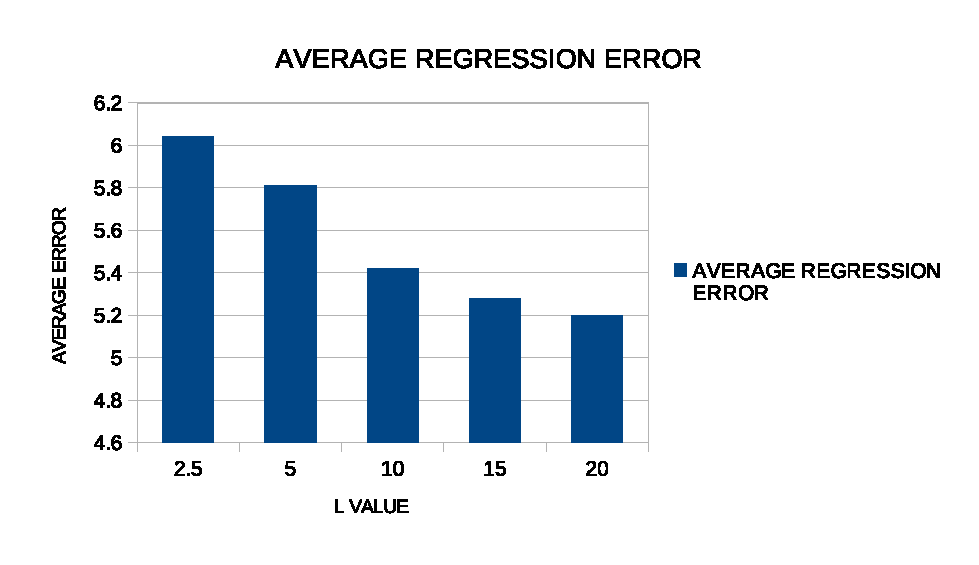
\includegraphics[scale=0.85]{lfactor}

\caption{Experiments with the $L$ parameter for the regression datasets. \label{fig:lfactor}}

\end{figure}
From the results, it is obvious that increasing the value of this
parameter also reduces the average error, but this reduction is not
extremely large to radically change the behavior of this technique.

In addition, corresponding experiments were performed with the value
of the coefficient $F$ increasing from 2 to 15 and these are graphically
illustrated in figure \ref{fig:ffactor}.
\begin{figure}[H]
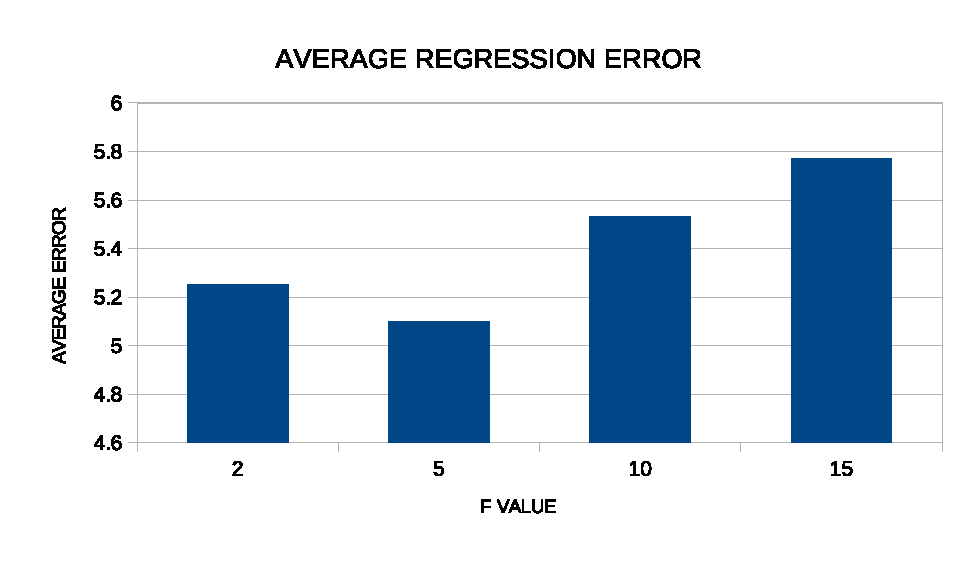
\includegraphics[scale=0.85]{ffactor}

\caption{Experiments with the value of parameter $F$ for the regression datasets.\label{fig:ffactor}}

\end{figure}
From these results it follows that the proposed method achieves the
best results for the value of the parameter to be equal to 5, although
again there is no significant difference in the effectiveness of the
method for large changes in the value of this parameter.

\section{Conclusions\label{sec:Conclusions}}

In this paper, a two-stage technique for efficient training of artificial
neural networks problems found in many scientific fields was presented.
During the first phase, a widely used global optimization technique
such as the Particle Swarm Optimization was used to minimize the training
error of the artificial neural network to which a penalty factor had
been added. This penalty factor is incorporated to maintain the effectiveness
of the artificial neural network to generalize to unknown data as
well. The calculation of the penalty factor is based on the observation
that the artificial neural network can lose its generalization abilities
when the input values in the sigmoid activation function exceed some
predetermined threshold. After the particle optimization technique
is performed in the second phase, the best particle is used both as
an initializer of a local optimization method and as a basis for calculating
bounds on the parameters of the artificial neural network.

The suggested method was applied to a wide range of classification
and regression problems found in the recentt literature and the experimental
results were more than encouraging. In addition, when comparing the
proposed technique with other widely used methods from the relevant
literature, it seems that the proposed technique significantly outperforms
them, especially in the case of regression problems. In relevant experiments
carried out regarding the sensitivity of the proposed technique on
its critical parameters, it was found to be quite robust without large
error fluctuations.

Future extensions of the technique may include its application to
other network cases such as Radial Basis Function artificial neural
networks (RBFs), as well as the use of global optimization methods
in the second stage of the proposed technique or even the creation
of appropriate termination techniques.

\vspace{6pt}


\authorcontributions{A.T. and I.G.T. conducted the experiments, employing several datasets
and provided the comparative experiments. D.T. and E.K. performed
the statistical analysis and prepared the manuscript. All authors
have read and agreed to the published version of the manuscript.}

\funding{This research received no external funding.}

\institutionalreview{Not applicable.}

\informedconsent{Not applicable. }

\institutionalreview{Not applicable.}

\acknowledgments{The experiments of this research work were performed at the high
performance computing system established at Knowledge and Intelligent
Computing Laboratory, Department of Informatics and Telecommunications,
University of Ioannina, acquired with the project “Educational Laboratory
equipment of TEI of Epirus” with MIS 5007094 funded by the Operational
Programme “Epirus” 2014--2020, by ERDF and national funds.}

\conflictsofinterest{The authors declare no conflict of interest.}

\sampleavailability{Not applicable.}

\appendixtitles{no}

\appendixstart{}

\appendix

\begin{adjustwidth}{-\extralength}{0cm}{}

\reftitle{References}
\begin{thebibliography}{99}
\bibitem{nn1}C. Bishop, Neural Networks for Pattern Recognition,
Oxford University Press, 1995.

\bibitem{nn2}G. Cybenko, Approximation by superpositions of a sigmoidal
function, Mathematics of Control Signals and Systems \textbf{2}, pp.
303-314, 1989.

\bibitem{nnphysics1}P. Baldi, K. Cranmer, T. Faucett et al, Parameterized
neural networks for high-energy physics, Eur. Phys. J. C \textbf{76},
2016.

\bibitem{nnphysics2}J. J. Valdas and G. Bonham-Carter, Time dependent
neural network models for detecting changes of state in complex processes:
Applications in earth sciences and astronomy, Neural Networks \textbf{19},
pp. 196-207, 2006

\bibitem{nnphysics3}G. Carleo,M. Troyer, Solving the quantum many-body
problem with artificial neural networks, Science \textbf{355}, pp.
602-606, 2017.

\bibitem{nnchem1}Lin Shen, Jingheng Wu, and Weitao Yang, Multiscale
Quantum Mechanics/Molecular Mechanics Simulations with Neural Networks,
Journal of Chemical Theory and Computation \textbf{12}, pp. 4934-4946,
2016.

\bibitem{nnchem2}Sergei Manzhos, Richard Dawes, Tucker Carrington,
Neural network‐based approaches for building high dimensional and
quantum dynamics‐friendly potential energy surfaces, Int. J. Quantum
Chem. \textbf{115}, pp. 1012-1020, 2015.

\bibitem{nnchem3}Jennifer N. Wei, David Duvenaud, and Alán Aspuru-Guzik,
Neural Networks for the Prediction of Organic Chemistry Reactions,
ACS Central Science \textbf{2}, pp. 725-732, 2016.

\bibitem{nnmed1}Igor I. Baskin, David Winkler and Igor V. Tetko,
A renaissance of neural networks in drug discovery, Expert Opinion
on Drug Discovery \textbf{11}, pp. 785-795, 2016.

\bibitem{nnmed2}Ronadl Bartzatt, Prediction of Novel Anti-Ebola Virus
Compounds Utilizing Artificial Neural Network (ANN), Chemistry Faculty
Publications \textbf{49}, pp. 16-34, 2018.

\bibitem{nnecon1}Lukas Falat and Lucia Pancikova, Quantitative Modelling
in Economics with Advanced Artificial Neural Networks, Procedia Economics
and Finance \textbf{34}, pp. 194-201, 2015.

\bibitem{nnecon2}Mohammad Namazi, Ahmad Shokrolahi, Mohammad Sadeghzadeh
Maharluie, Detecting and ranking cash flow risk factors via artificial
neural networks technique, Journal of Business Research \textbf{69},
pp. 1801-1806, 2016.

\bibitem{nnecon3}G. Tkacz, Neural network forecasting of Canadian
GDP growth, International Journal of Forecasting \textbf{17}, pp.
57-69, 2001.

\bibitem{nnde1}Y. Shirvany, M. Hayati, R. Moradian, Multilayer perceptron
neural networks with novel unsupervised training method for numerical
solution of the partial differential equations, Applied Soft Computing
\textbf{9}, pp. 20-29, 2009.

\bibitem{nnde2}A. Malek, R. Shekari Beidokhti, Numerical solution
for high order differential equations using a hybrid neural network---Optimization
method, Applied Mathematics and Computation \textbf{183}, pp. 260-271,
2006.

\bibitem{nnagr1}A. Topuz, Predicting moisture content of agricultural
products using artificial neural networks, Advances in Engineering
Software \textbf{41}, pp. 464-470, 2010.

\bibitem{nnagr2}A. Escamilla-García, G.M. Soto-Zarazúa, M. Toledano-Ayala,
E. Rivas-Araiza, A. Gastélum-Barrios, Abraham,Applications of Artificial
Neural Networks in Greenhouse Technology and Overview for Smart Agriculture
Development, Applied Sciences \textbf{10}, Article number 3835, 2020.

\bibitem{nnfacial}H. Boughrara, M. Chtourou, C. Ben Amar et al, Facial
expression recognition based on a mlp neural network using constructive
training algorithm. Multimed Tools Appl \textbf{75}, pp. 709--731,
2016.

\bibitem{nnwind}H. Liu, H.Q Tian, Y.F. Li, L. Zhang, Comparison of
four Adaboost algorithm based artificial neural networks in wind speed
predictions, Energy Conversion and Management \textbf{92}, pp. 67-81,
2015.

\bibitem{nngas}J. Szoplik, Forecasting of natural gas consumption
with artificial neural networks, Energy \textbf{85}, pp. 208-220,
2015.

\bibitem{nnintrusion}H. Bahram, N.J. Navimipour, Intrusion detection
for cloud computing using neural networks and artificial bee colony
optimization algorithm, ICT Express 5, pp. 56-59, 2019.

\bibitem{bpnn}D.E. Rumelhart, G.E. Hinton and R.J. Williams, Learning
representations by back-propagating errors, Nature \textbf{323}, pp.
533 - 536 , 1986.

\bibitem{bpnn2}T. Chen and S. Zhong, Privacy-Preserving Backpropagation
Neural Network Learning, IEEE Transactions on Neural Networks \textbf{20},
, pp. 1554-1564, 2009.

\bibitem{rpropnn}M. Riedmiller and H. Braun, A Direct Adaptive Method
for Faster Backpropagation Learning: The RPROP algorithm, Proc. of
the IEEE Intl. Conf. on Neural Networks, San Francisco, CA, pp. 586--591,
1993.

\bibitem{rpropnn3}T. Pajchrowski, K. Zawirski and K. Nowopolski,
Neural Speed Controller Trained Online by Means of Modified RPROP
Algorithm, IEEE Transactions on Industrial Informatics \textbf{11},
pp. 560-568, 2015.

\bibitem{rpropnn2}Rinda Parama Satya Hermanto, Suharjito, Diana,
Ariadi Nugroho, Waiting-Time Estimation in Bank Customer Queues using
RPROP Neural Networks, Procedia Computer Science \textbf{ 135}, pp.
35-42, 2018.

\bibitem{key-23}Neural Networks, Procedia Computer Science \textbf{ 135},
pp. 35-42, 2018.

\bibitem{quasinn}B. Robitaille and B. Marcos and M. Veillette and
G. Payre, Modified quasi-Newton methods for training neural networks,
Computers \& Chemical Engineering \textbf{20}, pp. 1133-1140, 1996.

\bibitem{quasinn2}Q. Liu, J. Liu, R. Sang, J. Li, T. Zhang and Q.
Zhang, Fast Neural Network Training on FPGA Using Quasi-Newton Optimization
Method,IEEE Transactions on Very Large Scale Integration (VLSI) Systems
\textbf{26}, pp. 1575-1579, 2018.

\bibitem{nn_ann1}A. Yamazaki, M. C. P. de Souto,T. B. Ludermir, Optimization
of neural network weights and architectures for odor recognition using
simulated annealing, In: Proceedings of the 2002 International Joint
Conference on Neural Networks. IJCNN'02 \textbf{1}, pp. 547-552 ,
2002.

\bibitem{nn_ann2}Y. Da, G. Xiurun, An improved PSO-based ANN with
simulated annealing technique, Neurocomputing \textbf{63}, pp. 527-533,
2005.

\bibitem{geneticnn}F. H. F. Leung, H. K. Lam, S. H. Ling and P. K.
S. Tam, Tuning of the structure and parameters of a neural network
using an improved genetic algorithm, IEEE Transactions on Neural Networks
\textbf{14}, pp. 79-88, 2003

\bibitem{geneticnn2}X. Yao, Evolving artificial neural networks,
Proceedings of the IEEE, 87(9), pp. 1423-1447, 1999.

\bibitem{psonn}C. Zhang, H. Shao and Y. Li, Particle swarm optimisation
for evolving artificial neural network, IEEE International Conference
on Systems, Man, and Cybernetics, , pp. 2487-2490, 2000.

\bibitem{psonn2}Jianbo Yu, Shijin Wang, Lifeng Xi, Evolving artificial
neural networks using an improved PSO and DPSO \textbf{71}, pp. 1054-1060,
2008.

\bibitem{nndem}J. Ilonen, J.K. Kamarainen, J. Lampinen, Differential
Evolution Training Algorithm for Feed-Forward Neural Networks, Neural
Processing Letters \textbf{17}, pp. 93--105, 2003.

\bibitem{nnevo}M. Rocha, P. Cortez, J. Neves, Evolution of neural
networks for classification and regression, Neurocomputing \textbf{70},
pp. 2809-2816, 2007.

\bibitem{nnwhale}I. Aljarah, H. Faris, S. Mirjalili, Optimizing connection
weights in neural networks using the whale optimization algorithm,
Soft Comput \textbf{22}, pp. 1--15, 2018.

\bibitem{nnbutterfly}S.M.J. Jalali, S. Ahmadian, P.M. Kebria, A.
Khosravi, C.P. Lim, S. Nahavandi, Evolving Artificial Neural Networks
Using Butterfly Optimization Algorithm for Data Classification. In:
Gedeon, T., Wong, K., Lee, M. (eds) Neural Information Processing.
ICONIP 2019. Lecture Notes in Computer Science(), vol 11953. Springer,
Cham, 2019.

\bibitem{nninit1}I. Ivanova, M. Kubat, Initialization of neural networks
by means of decision trees, Knowledge-Based Systems \textbf{8}, pp.
333-344, 1995.

\bibitem{nninit2}J.Y.F Yam, T.W.S. Chow, A weight initialization
method for improving training speed in feedforward neural network,
Neurocomputing \textbf{30}, pp. 219-232, 2000.

\bibitem{nninit3}F. Itano, M. A. de Abreu de Sousa, E. Del-Moral-Hernandez,
Extending MLP ANN hyper-parameters Optimization by using Genetic Algorithm,
In: 2018 International Joint Conference on Neural Networks (IJCNN),
Rio de Janeiro, Brazil, 2018, pp. 1-8, 2018.

\bibitem{nninit4}K. Chumachenko, A. Iosifidis, M. Gabbouj, Feedforward
neural networks initialization based on discriminant learning, Neural
Networks \textbf{146}, pp. 220-229, 2022.

\bibitem{nncross}R. Setiono, Feedforward Neural Network Construction
Using Cross Validation,Neural Computation \textbf{13}, pp. 2865-2877,
2001.

\bibitem{nnc}I.G. Tsoulos, D. Gavrilis, E. Glavas, Neural network
construction and training using grammatical evolution, Neurocomputing
72, pp. 269-277, 2008.

\bibitem{mainGe}M. O’Neill, C. Ryan, Grammatical evolution, IEEE
Trans. Evol. Comput. \textbf{5}, pp. 349--358, 2001.

\bibitem{nncell}K.J. Kim, S.B. Cho, Evolved neural networks based
on cellular automata for sensory-motor controller, Neurocomputing
\textbf{69}, pp. 2193-2207, 2006.

\bibitem{weight_gpu1}M. Martínez-Zarzuela, F.J. Díaz Pernas, J.F.
Díez Higuera, M.A. Rodríguez, Fuzzy ART Neural Network Parallel Computing
on the GPU. In: Sandoval, F., Prieto, A., Cabestany, J., Graña, M.
(eds) Computational and Ambient Intelligence. IWANN 2007. Lecture
Notes in Computer Science, vol 4507. Springer, Berlin, Heidelberg,
2007.

\bibitem{weight_gpu2}A.A. Huqqani, E. Schikuta, S. Ye Peng Chen,
Multicore and GPU Parallelization of Neural Networks for Face Recognition,
Procedia Computer Science \textbf{18}, pp. 349-358, 2013.

\bibitem{nnsharing1}S.J. Nowlan and G.E. Hinton, Simplifying neural
networks by soft weight sharing, Neural Computation 4, pp. 473-493,
1992.

\bibitem{nnsharing2}J.K. Kim, M.Y. Lee, J.Y. Kim, B. J. Kim, J. H.
Lee, An efficient pruning and weight sharing method for neural network,
In: 2016 IEEE International Conference on Consumer Electronics-Asia
(ICCE-Asia), Seoul, Korea (South), pp. 1-2, 2016.

\bibitem{nnprunning1}S.J. Hanson and L.Y. Pratt, Comparing biases
for minimal network construction with back propagation, In D.S. Touretzky
(Ed.), Advances in Neural Information Processing Systems, Volume 1,
pp. 177-185, San Mateo, CA: Morgan Kaufmann, 1989.

\bibitem{nnprunning2}M.C. Mozer and P. Smolensky, Skeletonization:
a technique for trimming the fat from a network via relevance assesment.
In D.S. Touretzky (Ed.), Advances in Neural Processing Systems, Volume
1, pp. 107-115, San Mateo CA: Morgan Kaufmann, 1989.

\bibitem{nnprunning3}M. Augasta and T. Kathirvalavakumar, Pruning
algorithms of neural networks --- a comparative study, Central European
Journal of Computer Science, 2003.

\bibitem{nndrop1}Nitish Srivastava, G E Hinton, Alex Krizhevsky,
Ilya Sutskever, Ruslan R Salakhutdinov, Dropout: a simple way to prevent
neural networks from overfitting, Journal of Machine Learning Research
\textbf{15}, pp. 1929-1958, 2014.

\bibitem{nndrop2}A. Iosifidis, A. Tefas, I. Pitas, DropELM: Fast
neural network regularization with Dropout and DropConnect, Neurocomputing
\textbf{162}, pp. 57-66, 2015.

\bibitem{nndecay1}A. Gupta, S.M. Lam, Weight decay backpropagation
for noisy data, Neural Networks \textbf{11}, pp. 1127-1138, 1998.

\bibitem{nndecay2}M. Carvalho and T. B. Ludermir, Particle Swarm
Optimization of Feed-Forward Neural Networks with Weight Decay, 2006
Sixth International Conference on Hybrid Intelligent Systems (HIS'06),
Rio de Janeiro, Brazil, 2006, pp. 5-5.

\bibitem{sarprop}N.K. Treadgold, T.D. Gedeon, Simulated annealing
and weight decay in adaptive learning: the SARPROP algorithm, IEEE
Trans. on Neural Networks 9, pp. 662-668, 1998.

\bibitem{nnpositive}M.D. Shahjahan, M. Kazuyuki, Neural network training
algorithm with possitive correlation, IEEE Trans. Inf \& Syst. \textbf{88},
pp. 2399-2409, 2005.

\bibitem{nngeman}S. Geman, E. Bienenstock and R. Doursat, Neural
networks and the bias/variance dilemma, Neural Computation 4 , pp.
1 - 58, 1992.

\bibitem{nnhawkins}Douglas M. Hawkins, The Problem of Overfitting,
J. Chem. Inf. Comput. Sci. \textbf{44}, pp. 1--12, 2004.

\bibitem{psoTutorial}F. Marini, B. Walczak, Particle swarm optimization
(PSO). A tutorial, Chemometrics and Intelligent Laboratory Systems
\textbf{149}, pp. 153-165, 2015.

\bibitem{psophysics1}Anderson Alvarenga de Moura Meneses, Marcelo
Dornellas, Machado Roberto Schirru, Particle Swarm Optimization applied
to the nuclear reload problem of a Pressurized Water Reactor, Progress
in Nuclear Energy \textbf{51}, pp. 319-326, 2009.

\bibitem{psophysics2}Ranjit Shaw, Shalivahan Srivastava, Particle
swarm optimization: A new tool to invert geophysical data, Geophysics
\textbf{72}, 2007.

\bibitem{psochem1}C. O. Ourique, E.C. Biscaia, J.C. Pinto, The use
of particle swarm optimization for dynamical analysis in chemical
processes, Computers \& Chemical Engineering \textbf{26}, pp. 1783-1793,
2002.

\bibitem{psochem2}H. Fang, J. Zhou, Z. Wang et al, Hybrid method
integrating machine learning and particle swarm optimization for smart
chemical process operations, Front. Chem. Sci. Eng. \textbf{16}, pp.
274--287, 2022.

\bibitem{psomed1}M.P. Wachowiak, R. Smolikova, Yufeng Zheng, J.M.
Zurada, A.S. Elmaghraby, An approach to multimodal biomedical image
registration utilizing particle swarm optimization, IEEE Transactions
on Evolutionary Computation \textbf{8}, pp. 289-301, 2004.

\bibitem{psomed2}Yannis Marinakis. Magdalene Marinaki, Georgios Dounias,
Particle swarm optimization for pap-smear diagnosis, Expert Systems
with Applications \textbf{35}, pp. 1645-1656, 2008. 

\bibitem{psoecon}Jong-Bae Park, Yun-Won Jeong, Joong-Rin Shin, Kwang
Y. Lee, An Improved Particle Swarm Optimization for Nonconvex Economic
Dispatch Problems, IEEE Transactions on Power Systems \textbf{25},
pp. 156-16\textbf{216}6, 2010.

\bibitem{pso_major}J. Kennedy and R. Eberhart, \textquotedbl Particle
swarm optimization,\textquotedbl{} Proceedings of ICNN'95 - International
Conference on Neural Networks, 1995, pp. 1942-1948 vol.4, doi: 10.1109/ICNN.1995.488968.

\bibitem{random_inertia}R.C. Eberhart, Y.H. Shi, Tracking and optimizing
dynamic systems with particle swarms, in: Congress on Evolutionary
Computation, Korea, 2001.

\bibitem{inertia1} Y.H. Shi, R.C. Eberhart, Empirical study of particle
swarm optimization, in: Congress on Evolutionary Computation, Washington
DC, USA, 1999. 

\bibitem{inertia2}Y.H. Shi, R.C. Eberhart, Experimental study of
particle swarm optimization, in: SCI2000 Conference, Orlando, 2000.

\bibitem{Powell}M.J.D Powell, A Tolerant Algorithm for Linearly Constrained
Optimization Calculations, Mathematical Programming \textbf{45}, pp.
547-566, 1989. 

\bibitem{bfgs2}R. Fletcher, A new approach to variable metric algorithms,
Computer Journal \textbf{13}, pp. 317-322, 1970. 

\bibitem{Keel}J. Alcalá-Fdez, A. Fernandez, J. Luengo, J. Derrac,
S. García, L. Sánchez, F. Herrera. KEEL Data-Mining Software Tool:
Data Set Repository, Integration of Algorithms and Experimental Analysis
Framework. Journal of Multiple-Valued Logic and Soft Computing 17,
pp. 255-287, 2011.

\bibitem{appendicitis}Weiss, Sholom M. and Kulikowski, Casimir A.,
Computer Systems That Learn: Classification and Prediction Methods
from Statistics, Neural Nets, Machine Learning, and Expert Systems,
Morgan Kaufmann Publishers Inc, 1991.

\bibitem{australian}J.R. Quinlan, Simplifying Decision Trees. International
Journal of Man-Machine Studies \textbf{27}, pp. 221-234, 1987. 

\bibitem{balance}T. Shultz, D. Mareschal, W. Schmidt, Modeling Cognitive
Development on Balance Scale Phenomena, Machine Learning \textbf{16},
pp. 59-88, 1994.

\bibitem{cleveland1}Z.H. Zhou,Y. Jiang, NeC4.5: neural ensemble based
C4.5,\textquotedbl{} in IEEE Transactions on Knowledge and Data Engineering
\textbf{16}, pp. 770-773, 2004.

\bibitem{cleveland2}R. Setiono , W.K. Leow, FERNN: An Algorithm for
Fast Extraction of Rules from Neural Networks, Applied Intelligence
\textbf{12}, pp. 15-25, 2000.

\bibitem{dermatology}G. Demiroz, H.A. Govenir, N. Ilter, Learning
Differential Diagnosis of Eryhemato-Squamous Diseases using Voting
Feature Intervals, Artificial Intelligence in Medicine. \textbf{13},
pp. 147--165, 1998.

\bibitem{heart}I. Kononenko, E. Šimec, M. Robnik-Šikonja, Overcoming
the Myopia of Inductive Learning Algorithms with RELIEFF, Applied
Intelligence \textbf{7}, pp. 39--55, 1997

\bibitem{hayesroth}B. Hayes-Roth, B., F. Hayes-Roth. Concept learning
and the recognition and classification of exemplars. Journal of Verbal
Learning and Verbal Behavior \textbf{16}, pp. 321-338, 1977.

\bibitem{housevotes}R.M. French, N. Chater, Using noise to compute
error surfaces in connectionist networks: a novel means of reducing
catastrophic forgetting, Neural Comput. \textbf{14}, pp. 1755-1769,
2002.

\bibitem{ion1}J.G. Dy , C.E. Brodley, Feature Selection for Unsupervised
Learning, The Journal of Machine Learning Research \textbf{5}, pp
845--889, 2004.

\bibitem{ion2}S. J. Perantonis, V. Virvilis, Input Feature Extraction
for Multilayered Perceptrons Using Supervised Principal Component
Analysis, Neural Processing Letters \textbf{10}, pp 243--252, 1999.

\bibitem{liver} J. Garcke, M. Griebel, Classification with sparse
grids using simplicial basis functions, Intell. Data Anal. \textbf{6},
pp. 483-502, 2002.

\bibitem{mammographic}M. Elter, R. Schulz-Wendtland, T. Wittenberg,
The prediction of breast cancer biopsy outcomes using two CAD approaches
that both emphasize an intelligible decision process, Med Phys. \textbf{34},
pp. 4164-72, 2007.

\bibitem{pageblocks}F. Esposito F., D. Malerba, G. Semeraro, Multistrategy
Learning for Document Recognition, Applied Artificial Intelligence
\textbf{8}, pp. 33-84, 1994. 

\bibitem{parkinsons}M.A. Little, P.E. McSharry, E.J. Hunter, J. Spielman,
L.O. Ramig, Suitability of dysphonia measurements for telemonitoring
of Parkinson's disease. IEEE Trans Biomed Eng. \textbf{56}, pp. 1015-1022,
2009.

\bibitem{pima}J.W. Smith, J.E. Everhart, W.C. Dickson, W.C. Knowler,
R.S. Johannes, Using the ADAP learning algorithm to forecast the onset
of diabetes mellitus, In: Proceedings of the Symposium on Computer
Applications and Medical Care IEEE Computer Society Press, pp.261-265,
1988.

\bibitem{popfailures}D.D. Lucas, R. Klein, J. Tannahill, D. Ivanova,
S. Brandon, D. Domyancic, Y. Zhang, Failure analysis of parameter-induced
simulation crashes in climate models, Geoscientific Model Development
\textbf{6}, pp. 1157-1171, 2013.

\bibitem{regions}N. Giannakeas, M.G. Tsipouras, A.T. Tzallas, K.
Kyriakidi, Z.E. Tsianou, P. Manousou, A. Hall, E.C. Karvounis, V.
Tsianos, E. Tsianos, A clustering based method for collagen proportional
area extraction in liver biopsy images (2015) Proceedings of the Annual
International Conference of the IEEE Engineering in Medicine and Biology
Society, EMBS, 2015-November, art. no. 7319047, pp. 3097-3100. 

\bibitem{saheart}T. Hastie, R. Tibshirani, Non-parametric logistic
and proportional odds regression, JRSS-C (Applied Statistics) \textbf{36},
pp. 260--276, 1987.

\bibitem{segment}M. Dash, H. Liu, P. Scheuermann, K. L. Tan, Fast
hierarchical clustering and its validation, Data \& Knowledge Engineering
\textbf{44}, pp 109--138, 2003.

\bibitem{wdbc}W.H. Wolberg, O.L. Mangasarian, Multisurface method
of pattern separation for medical diagnosis applied to breast cytology,
Proc Natl Acad Sci U S A. \textbf{87}, pp. 9193--9196, 1990.

\bibitem{wine1}M. Raymer, T.E. Doom, L.A. Kuhn, W.F. Punch, Knowledge
discovery in medical and biological datasets using a hybrid Bayes
classifier/evolutionary algorithm. IEEE transactions on systems, man,
and cybernetics. Part B, Cybernetics : a publication of the IEEE Systems,
Man, and Cybernetics Society, \textbf{33} , pp. 802-813, 2003.

\bibitem{wine2}P. Zhong, M. Fukushima, Regularized nonsmooth Newton
method for multi-class support vector machines, Optimization Methods
and Software \textbf{22}, pp. 225-236, 2007.

\bibitem{zoo}M. Koivisto, K. Sood, Exact Bayesian Structure Discovery
in Bayesian Networks, The Journal of Machine Learning Research\textbf{
5}, pp. 549--573, 2004.

\bibitem{key-20}R.G. Andrzejak, K. Lehnertz, F. Mormann, C. Rieke,
P. David, and C. E. Elger, Indications of nonlinear deterministic
and finite-dimensional structures in time series of brain electrical
activity: Dependence on recording region and brain state, Phys. Rev.
E \textbf{64}, pp. 1-8, 2001.

\bibitem{abalone}W. J Nash, T.L. Sellers, S.R. Talbot, A.J. Cawthor,
W.B. Ford, The Population Biology of Abalone (\_Haliotis\_ species)
in Tasmania. I. Blacklip Abalone (\_H. rubra\_) from the North Coast
and Islands of Bass Strait, Sea Fisheries Division, Technical Report
No. 48 (ISSN 1034-3288), 1994.

\bibitem{airfoil}T.F. Brooks, D.S. Pope, A.M. Marcolini, Airfoil
self-noise and prediction. Technical report, NASA RP-1218, July 1989. 

\bibitem{Stat}J.S. Simonoff, Smooting Methods in Statistics, Springer
- Verlag, 1996.

\bibitem{concrete}I.Cheng Yeh, Modeling of strength of high performance
concrete using artificial neural networks, Cement and Concrete Research.
\textbf{28}, pp. 1797-1808, 1998. 

\bibitem{key23}D. Harrison and D.L. Rubinfeld, Hedonic prices and
the demand for clean ai, J. Environ. Economics \& Management \textbf{5},
pp. 81-102, 1978.

\bibitem{key21}J.S. Simonoff, Smooting Methods in Statistics, Springer
- Verlag, 1996.

\bibitem{pydataset}R.D. King, S. Muggleton, R. Lewis, M.J.E. Sternberg,
Proc. Nat. Acad. Sci. USA \textbf{89}, pp. 11322--11326, 1992. 

\bibitem{Adam}D. P. Kingma, J. L. Ba, ADAM: a method for stochastic
optimization, in: Proceedings of the 3rd International Conference
on Learning Representations (ICLR 2015), pp. 1--15, 2015.

\bibitem{fcn}Grzegorz Klima, Fast Compressed Neural Networks, available
from \url{http://fcnn.sourceforge.net/}.

\bibitem{neat}K. O. Stanley, R. Miikkulainen, Evolving Neural Networks
through Augmenting Topologies, Evolutionary Computation \textbf{10},
pp. 99-127, 2002.

\end{thebibliography}

\end{adjustwidth}{}
\end{document}
